\documentclass[12pt,a4paper]{article}
\usepackage[utf8]{inputenc}
\usepackage[spanish]{babel}
\usepackage{amsmath}
\usepackage{amsfonts}
\usepackage{amssymb}
\usepackage{cancel}
\usepackage{graphicx}
\usepackage[left=2cm,right=2cm,top=2cm,bottom=2cm]{geometry}
\author{Federico Almada}
\begin{document}
\begin{titlepage}
	\includegraphics[width=6cm]{unaj.jpg}
    \centering
    \vfill
    \Huge \textbf{Trabajo Práctico Final}
    \vskip2cm
    \Large Complejidad Temporal, Estructura de datos y Algoritmos\\
    Primer cuatrimestre de 2020\\
    Comisión 05 - Prof. Leonardo Amet     
    \vfill
    \begin{tabular}{ | l | l | l}
      \hline
      Alumno: & Almada, Federico \\ \hline
      Número de legajo: & 27787 \\ \hline
      Email: & federico.almada1998@gmail.com \\ \hline
      DNI: & 41.136.004 \\ \hline
  	\end{tabular}
    \vfill
    \vfill
\end{titlepage}
\newpage
\tableofcontents
\newpage

\section{Introducción}
El presente informe es para el Trabajo Práctico Final de la materia Complejidad Temporal, Estructura de datos y Algoritmos que consiste en desarrollar un juego de cartas entre dos contrincantes (el usuario y la computadora). El objetivo principal del mismo es programar la Inteligencia Artificial (IA) con la cual la computadora va a elegir sus cartas, esto se hará mediante un árbol MiniMax.

\subsection{Objetivos generales}
\begin{itemize}
	\item Implementar el armado del árbol de decisiones.
	\item Desarrollar la estrategia con la que la IA tomará decisiones favorables.
	\item Desarrollar la metodología con la que la IA irá descartando sus cartas.
	\item Presentar el desarrollo del trabajo así como también los problemas hallados y sus soluciones.
\end{itemize}
\newpage
\section{Descripción del juego}
Básicamente es un 1 vs 1 entre dos jugadores, primero juega el usuario y luego es el turno de la computadora. El juego consta de  un mazo de 12 cartas enumereadas del 1 al 12, a cada participante le corresponde 6 cartas aleatorias del mazo. También, el juego establece un límite al azar entre un rango especificado. A medida que los jugadores van descartando sus cartas, se forma un montículo en donde se sumaran todas las cartas descartadas, el jugador que pierde será el que tire la carta que haga que el montículo supere el límite asignado.  

\section{Algoritmo MiniMax}
En resumidas palabras, consiste en la elección del mejor movimiento para la computadora, suponiendo que el usuario elegirá uno que le pueda perjudicar. Para elegir la mejor opción este algoritmo realiza un árbol de búsqueda con todos los posibles movimientos, luego recorre todo el árbol de soluciones del juego a partir de un estado dado, es decir, a partir de una jugada realizada. Por lo tanto, este algoritmo será ejecutado cada vez que juegue la computadora.\\

En el caso actual, este algorimo le será muy útil a la computadora para ir descartando cartas cuando sea su turno, ya que de antemano sabrá cuales son sus mejores jugadas y por cual camino tendrá más posibilidades de ganar.\\

Para saber que jugada le conviene o no a la computadora, existe una estrategia o funcion heuristica que indica cual jugada es más conveniente hacer, si la funcion heuristica tiene un valor alto, entonces le conviene a la computadora, en caso contrario, le conviene al oponente.

\section{Diagrama de clases UML}
\begin{center}
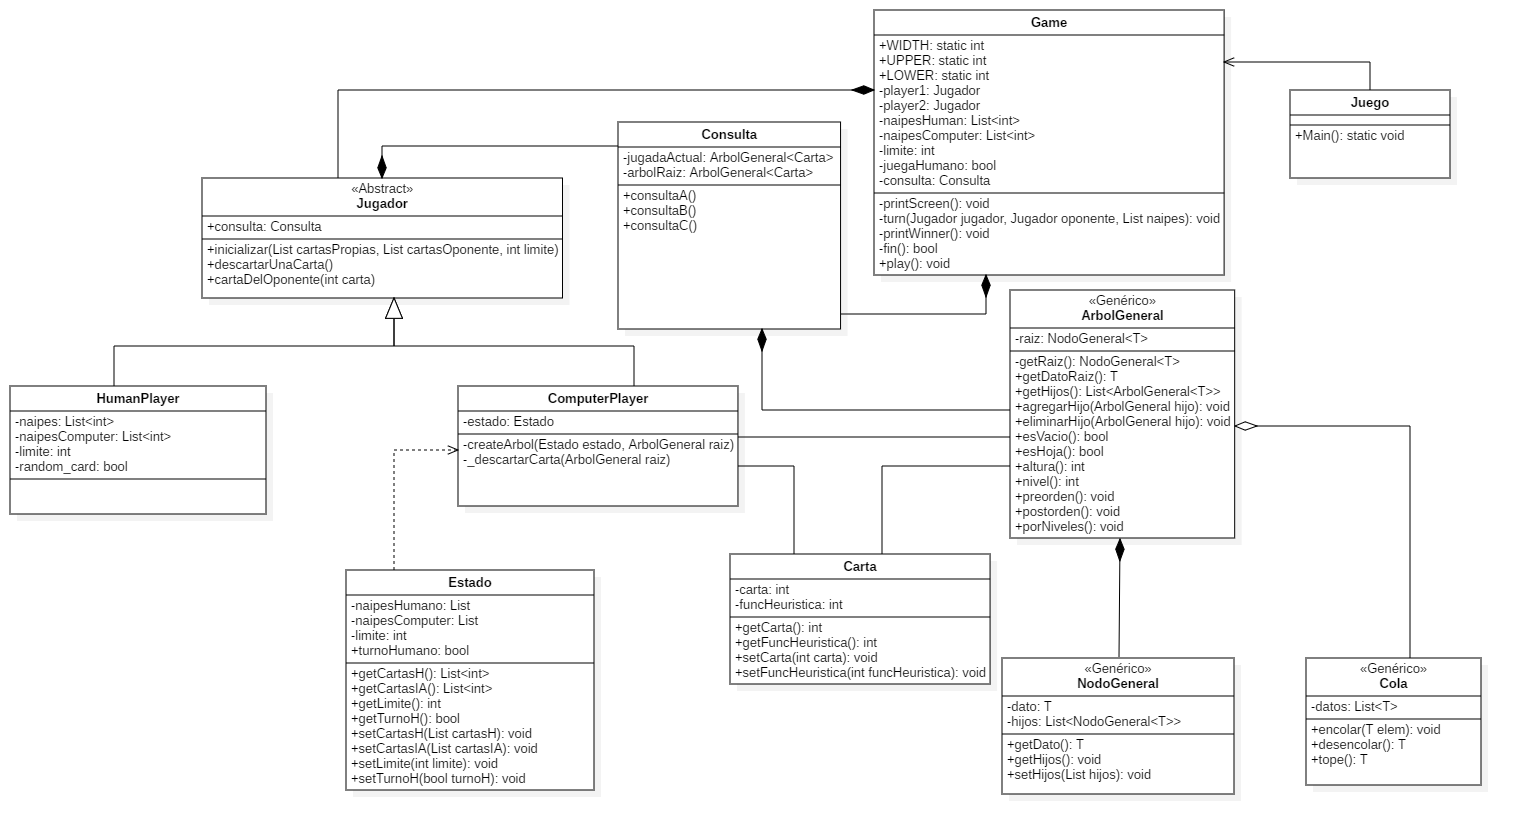
\includegraphics[scale=0.32]{diagrama_UML.png} 
\end{center}

En la clase Estado se almacena cada estado o jugada que será necesaria para ir armando el árbol de decisiones, por lo que depende del estado de la jugada de la clase ComputerPlayer.
Por otro lado, la clase Consulta es la que tiene todos los métodos necesarios con los cuales el usuario en cada momento del juego podrá solicitar una funcionalidad para ver el desarrollo del arbol en cualquier jugada del árbol de soluciones.
\newpage
\section{Problemas encontrados}
Durante el desarrollo del juego surgieron distintos problemas, por un lado, el mayor de los problemas fue la hora de la creación del árbol de posibilidades, en el método Inicializar de la clase ComputerPlayer. Por otro lado, en el mismo método, también ocurrieron algunos problemas en relación a la asignación de la función heuristica. 

\subsection{Soluciones de problemas}
Para solucionar el armado del arbol, lo que se hizo fue crear un algoritmo recursivo que permita armar el arbol lo más eficiente posible, de tal forma que se pare con el armado del árbol cuando se llegue a un caso base. El caso es cuando se llega a un nodo o carta, donde el límite del juego sea menos a 0.
Por otro lado, en relación a la asignación de la función heuristica, a medida que el árbol de decisiones vuelve de la recursión, se realizó un booleano que, dependiendo el valor heuristico de los nodos hijos de cada nodo raiz, se maximiza o minimiza su valor de función heuristica. Cuando sea el turno de la IA se maximiza el resultado, y cuando sea el turno de la computadora se minimiza su resultado.


\section{Interfaz del juego}
\begin{center}
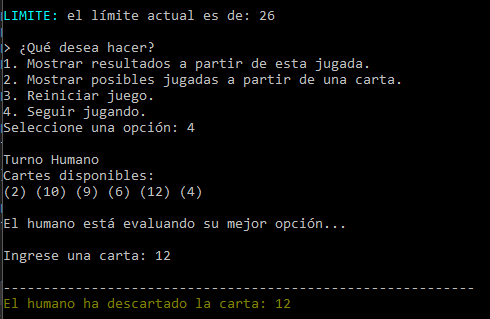
\includegraphics[scale=0.7]{captura1.PNG} 
\end{center}
Como se pude observar, primero se asigna un límite al azar, entre un rango determinado por el juego. El humano va a tener en cada jugada la posibilidad de hacer una consulta. Cuando el humano descarta su carta, se invierte el turno y la IA utiliza la función heuristica para decidir cual será su mejor opción. Como se puede ver en la siguiente captura, el color verde indica que es una buena jugada para la computadora, por el contrario, el color rojo indicia que es una buena jugada para el usuario. El usuario tiene la posibilidad de reiniciar el juego cuando lo desee.

\begin{center}
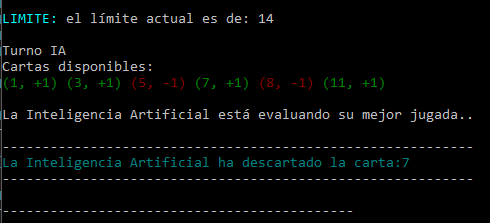
\includegraphics[scale=0.7]{captura2.PNG} 
\end{center}

\section{Consultas}
El jugador cada vez que juega tiene disponible 3 consultas.
\begin{itemize}
\item Imprimir posibles resultados a partir de un punto, es decir, los caminos que se forman a partir de un nodo raiz hasta una hoja.
\item Escribir una secuencia de cartas y simular las jugadas para ver que pasaría a partir de ese punto.
\item Mostrar todas las cartas a partir de un cierto nivel de profundidad.
\end{itemize}

También, el usuario dispone de 3 utilizades:
\begin{itemize}
\item Salir del juego.
\item Seguir jugando.
\item Reiniciar una partida.
\end{itemize}
\begin{center}
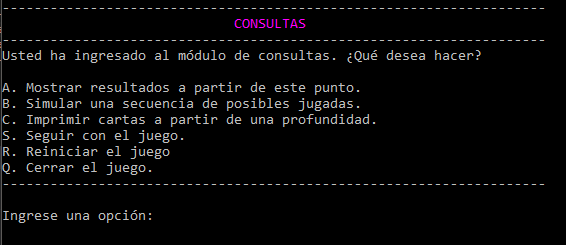
\includegraphics[scale=0.7]{captura3.PNG} 
\end{center}
\subsection{Consulta A}
Si el usuario presiona la tecla A, se muestra consulta que imprime todos los caminos posibles a partir de un cierto punto. 
\subsection{Consulta B}
Si el usuario presiona la tecla C, podrá simular una secuencia de cartas y avanzar para comprobar que pasará en cierto punto.
Vale aclarar que al ser una partida simulada, no afectará a la jugada original.
\subsection{Consulta C}
Si el usuario presiona la tecla C, se hace un recorrido por niveles y se imprime en pantalla un nivel completo con las cartas, si aparece en color celeste, es del humano, sino de la IA.
\begin{center}
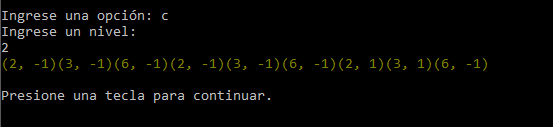
\includegraphics[scale=0.8]{captura4.PNG} 
\end{center}
\newpage
\section{Mejoras}
Para mejorar la experiencia para el usuario, se le ha asignado un Timer desde un rango entre 1,5 seg y 5 seg al descarte de carta de la Inteligencia Articial para aparentar que está pensando en que carta lanzar.Una mejora posible para el juego podría ser que el turno de los jugadores se invierta cuando el usuario lo desee, o sino, que sea elegido aleatoriamente por el juego. También sería ideal implementar un sistema de dificultades para que la IA le de más oportunidades de ganar al usuario. Por ejemplo, que exista una dificultad 'Normal' en donde la computadora tenga solo un 60 porciento de posibilidades de ganar.

\section{Conclusiones}
En conclusión, los distintos problemas que fueron surgiendo en la implementación se pudieron solucionar, luego fue mas sencillo seguir con el desarrollo del juego.\\

Quedó demostrado que con el algoritmo MiniMax, la IA gana en la mayoría de los casos, sin embargo, hay ciertas ocaciones en donde si el humano juega bien puede llegar a ganar.\\

Para mejorar la eficiencia del árbol de decisiones se decidió hacer un caso donde que permita frenar el armado del árbol MiniMax.\\

Por último, el trabajo fue de mucha utilidad para solidificar los conceptos aprendidos durante el transcurso de la cursada.
\newpage
\section{Bibliografía}
[1] Devcode.la - "\emph{El algoritmo Minimax y su aplicación en un juego}"\\
https://devcode.la/tutoriales/algoritmo-minimax
\end{document}
